\chapter{Hito 5: Monitorización, feedback loop y shadow testing}
\label{chap:hito5}

\section{Introducción}

El quinto hito del proyecto tiene como objetivo ampliar el sistema desplegado en el Hito 4 con capacidades de observabilidad, monitorización y mejora continua propias de un flujo MLOps. Para ello, se ha diseñado una solución orientada a supervisar el comportamiento operativo del servicio, detectar posibles signos de degradación del modelo en producción y cerrar el ciclo mediante un mecanismo de realimentación y reentrenamiento.

A diferencia de los hitos anteriores, en esta fase el foco no se sitúa únicamente en desplegar un modelo funcional, sino en dotar al sistema de herramientas que permitan operar con mayor seguridad una vez puesto en servicio. En particular, se ha abordado el problema de cómo monitorizar un clasificador cuando la etiqueta real de cada muestra no está disponible en el instante de la predicción, situación habitual en escenarios reales de explotación.

En el contexto de VinOps, la clase real del cultivar no puede conocerse en tiempo real, ya que su validación depende de la revisión posterior del enólogo. Esta restricción impide calcular de manera inmediata métricas clásicas de rendimiento como el F1-score, la precisión o el AUC. Por este motivo, en este hito se ha optado por complementar la inferencia con métricas proxy, detección de drift, alertas automáticas y un mecanismo de feedback que permita incorporar correcciones humanas al ciclo de vida del modelo.

Además del desarrollo técnico, este capítulo pone el foco en las decisiones de diseño adoptadas para mantener una solución ligera, reproducible y coherente con el carácter académico del proyecto. Se justifica por qué se ha optado por determinadas herramientas y estrategias, y se analizan las implicaciones que dichas decisiones han tenido sobre la mantenibilidad, la interpretabilidad y la operatividad del sistema.

\section{Arquitectura general del sistema de observabilidad}

La arquitectura implementada extiende el servicio de inferencia desarrollado en el hito anterior mediante una capa adicional de instrumentación, trazabilidad y supervisión. El sistema se articula alrededor de una API desarrollada con FastAPI, accesible en el puerto 8001, que expone tanto el endpoint de predicción como varios endpoints auxiliares orientados a la monitorización, el feedback y el reentrenamiento.

A nivel funcional, cuando un cliente envía una muestra a \texttt{/predict}, el sistema realiza la inferencia, calcula métricas proxy de calidad de la predicción, evalúa si la entrada presenta rasgos anómalos respecto a la distribución de entrenamiento, registra la ejecución en un log estructurado y actualiza las métricas expuestas para Prometheus. Sobre esta base, Grafana permite visualizar el comportamiento del servicio, mientras que un sistema de alertas por Telegram notifica situaciones relevantes al equipo.

La solución se ha desacoplado del despliegue del Hito 4 mediante una carpeta específica de observabilidad. Esta decisión permite mantener separado el sistema base de inferencia del entorno ampliado de monitorización, facilitando la revisión académica y evitando introducir complejidad innecesaria sobre el despliegue mínimo ya validado.

De forma general, los endpoints principales del servicio son los siguientes:

\begin{table}[h]
\centering
\caption{Endpoints principales del sistema monitorizado}
\vspace{0.2cm}
\begin{tabular}{l l p{8.2cm}}
\hline
\textbf{Endpoint} & \textbf{Método} & \textbf{Función principal} \\
\hline
\texttt{/health} & GET & Verificar el estado del servicio, exponer metadatos básicos del modelo y resumir información operativa. \\
\texttt{/predict} & POST & Realizar la predicción, calcular métricas proxy, detectar anomalías y registrar la inferencia. \\
\texttt{/metrics} & GET & Exponer las métricas en formato Prometheus para su recolección externa. \\
\texttt{/monitor} & GET & Consultar un resumen agregado de actividad, anomalías y calidad de predicción. \\
\texttt{/feedback} & POST & Registrar correcciones proporcionadas por el enólogo para alimentar el ciclo de mejora. \\
\texttt{/retrain} & POST & Lanzar un reentrenamiento a partir del dataset original y del feedback acumulado. \\
\texttt{/reload} & POST & Recargar en memoria el modelo actualizado sin reiniciar el contenedor. \\
\hline
\end{tabular}
\label{tab:endpoints_hito5}
\end{table}

Como ampliación opcional, se ha implementado también un entorno de \textit{shadow testing} en un puerto independiente, orientado a comparar un modelo en producción con un modelo candidato sin afectar a la respuesta devuelta al cliente. Esta extensión se comenta más adelante como bonus del hito.

Las Figuras~\ref{fig:h5_docker_stack} y~\ref{fig:h5_health_main} ilustran tanto el despliegue efectivo del entorno como la disponibilidad del servicio principal.

\begin{figure}[H]
\centering
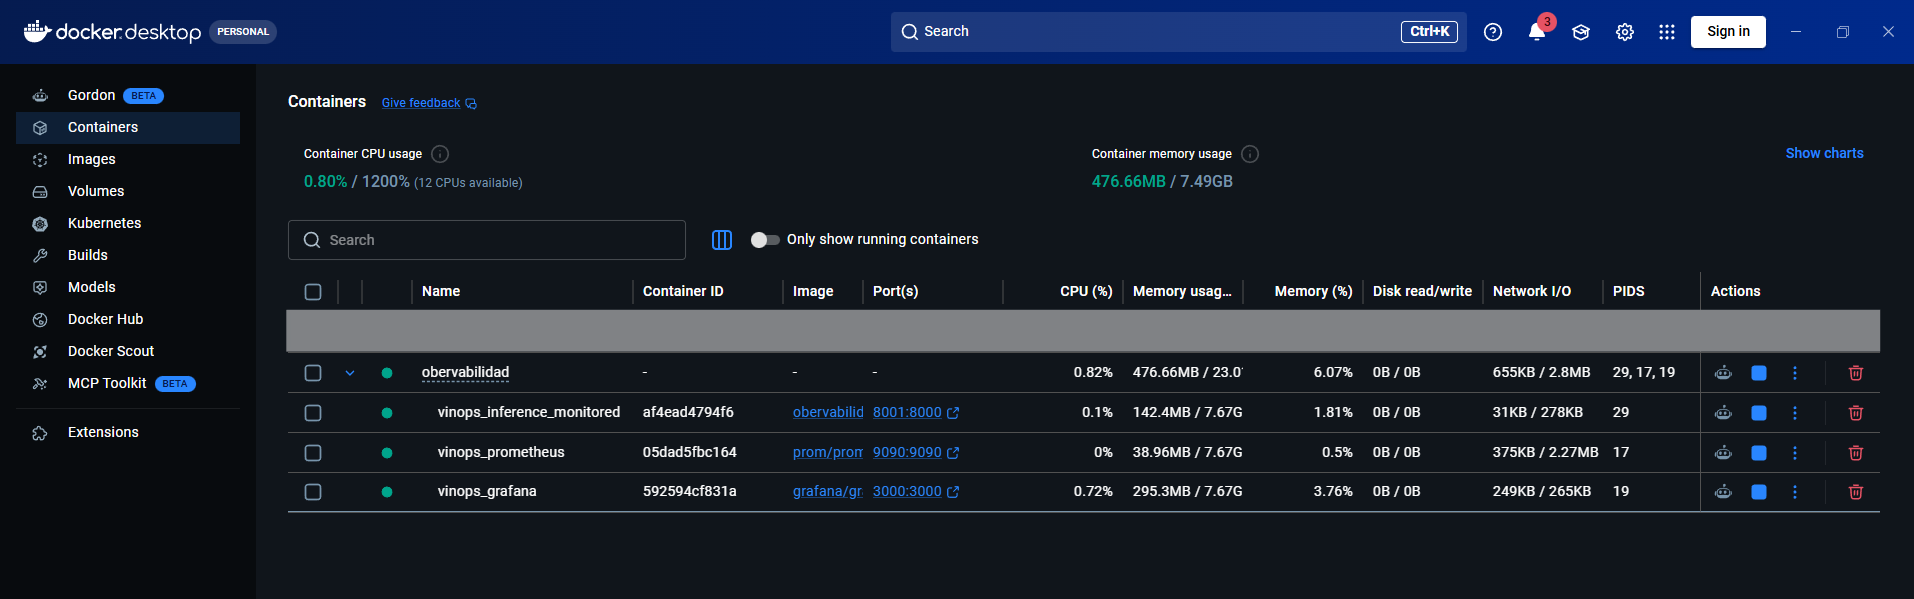
\includegraphics[width=0.96\textwidth]{Pictures/dockerdesktop.png}
\caption{Entorno de observabilidad desplegado en Docker con la API monitorizada y los servicios auxiliares activos.}
\label{fig:h5_docker_stack}
\end{figure}

\begin{figure}[H]
\centering
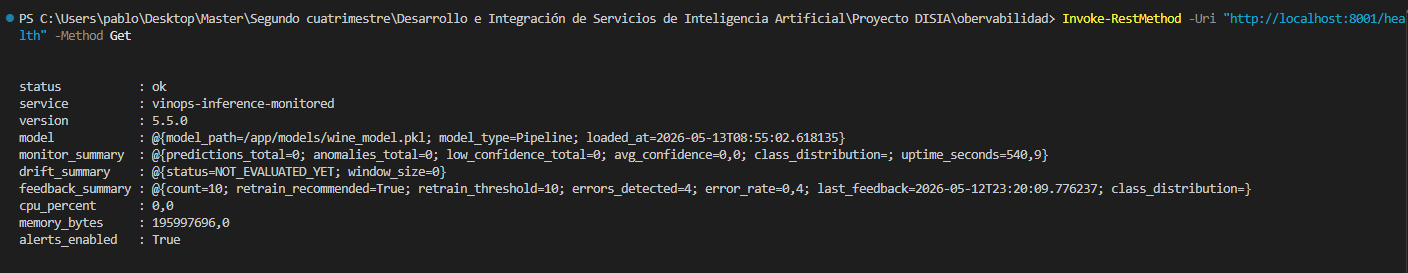
\includegraphics[width=0.95\textwidth]{Pictures/llamada API puerto 8001.png}
\caption{Respuesta del endpoint \texttt{/health} del servicio principal en el puerto 8001.}
\label{fig:h5_health_main}
\end{figure}

\FloatBarrier

\section{Instrumentación y trazabilidad del servicio}

Uno de los objetivos centrales del hito ha sido convertir la API de inferencia en un servicio observable. Para ello, se han instrumentado métricas operativas habituales en sistemas software, tales como número de peticiones, latencia, uso de CPU y consumo de memoria. Esta instrumentación permite supervisar no solo el comportamiento del modelo, sino también el estado general del servicio que lo ejecuta.

La elección de Prometheus como solución de monitorización responde a varias razones. En primer lugar, se trata de una herramienta utilizada en entornos cloud-native y con integración nativa con Grafana. En segundo lugar, el cliente de Python resulta ligero y sencillo de integrar en FastAPI. Finalmente, el formato textual de las métricas facilita tanto la depuración como la validación manual durante una demostración académica.

Las principales métricas operativas instrumentadas han sido las presentados en la Tabla \ref{tab:metricas_operativas_hito5}.

\begin{table}[h]
\centering
\caption{Métricas operativas instrumentadas}
\vspace{0.2cm}
\begin{tabular}{l l p{7.5cm}}
\hline
\textbf{Métrica} & \textbf{Tipo} & \textbf{Descripción} \\
\hline
\texttt{vinops\_requests\_total} & Counter & Cuenta peticiones HTTP por método, endpoint y código de estado. \\
\texttt{vinops\_request\_latency\_seconds} & Histogram & Mide la latencia de las peticiones, especialmente en inferencia. \\
\texttt{vinops\_cpu\_usage\_percent} & Gauge & Registra el uso de CPU del proceso que ejecuta el servicio. \\
\texttt{vinops\_memory\_usage\_bytes} & Gauge & Registra el consumo de memoria residente del proceso. \\
\hline
\end{tabular}
\label{tab:metricas_operativas_hito5}
\end{table}

Junto a las métricas operativas, se ha considerado necesario instrumentar también métricas proxy del modelo. La razón es que, en el dominio del proyecto, la etiqueta real no está disponible en el instante de la predicción, por lo que no es posible calcular online métricas de rendimiento supervisadas. En consecuencia, se ha optado por monitorizar señales indirectas que permitan detectar comportamientos sospechosos antes de disponer del \textit{ground truth}.

Entre estas métricas proxy, presentadas en la Tabla \ref{tab:metricas_proxy_hito5}, destacan la confianza de la predicción, la entropía de la distribución de probabilidades, el conteo de predicciones por clase, la tasa de muestras anómalas y el número de predicciones con confianza baja. La confianza y la entropía resultan especialmente útiles porque permiten detectar cuándo el modelo se encuentra en una zona de mayor incertidumbre, algo relevante en este problema debido al solapamiento ya observado entre algunas clases en el Hito 3.

\begin{table}[h]
\centering
\caption{Métricas proxy del modelo}
\vspace{0.2cm}
\begin{tabular}{l l p{7.2cm}}
\hline
\textbf{Métrica} & \textbf{Tipo} & \textbf{Interpretación} \\
\hline
\texttt{vinops\_prediction\_confidence} & Histogram & Mide la probabilidad máxima asignada por el modelo a la clase predicha. \\
\texttt{vinops\_prediction\_entropy} & Histogram & Evalúa el grado de dispersión de la distribución de probabilidades entre clases. \\
\texttt{vinops\_predictions\_by\_class\_total} & Counter & Permite analizar cambios en la distribución de clases predichas. \\
\texttt{vinops\_anomaly\_flags\_total} & Counter & Cuenta las muestras detectadas como anómalas respecto a la referencia. \\
\texttt{vinops\_low\_confidence\_total} & Counter & Cuenta predicciones cuya confianza cae por debajo del umbral establecido. \\
\hline
\end{tabular}
\label{tab:metricas_proxy_hito5}
\end{table}

Otra decisión de diseño relevante ha sido reutilizar en inferencia la lógica de detección de anomalías introducida en el Hito 2. Para cada muestra entrante se calcula el z-score de cada variable respecto a la media y desviación estándar del conjunto de entrenamiento, siguiendo la expresión:

\[
z_j = \frac{x_j - \bar{x}_j}{\sigma_j}, \qquad j = 1,\ldots,13
\]

Si alguna variable supera en valor absoluto el umbral de tres desviaciones estándar, la muestra se marca como anómala. Esta estrategia aporta coherencia entre el análisis exploratorio previo y la supervisión operativa del sistema, además de ofrecer una forma simple y explicable de identificar entradas poco representativas.

La trazabilidad de las predicciones se completa mediante un sistema de \textit{logging} estructurado en formato JSONL. Cada inferencia genera una línea independiente que incluye el instante temporal, las variables de entrada, la clase predicha, las probabilidades por clase, la confianza, la entropía, el resultado del detector de anomalías y la latencia de la respuesta. Se ha optado por JSONL porque permite escritura incremental eficiente sin necesidad de reescribir estructuras completas, y facilita el análisis posterior con herramientas de línea de comandos o librerías como \texttt{pandas}.

Las Figuras~\ref{fig:h5_predict_normal} y~\ref{fig:h5_predict_anomalous} ilustran dos situaciones representativas del servicio de inferencia: una predicción ordinaria con comportamiento esperado y una muestra con rasgos anómalos detectados por el monitor.

\begin{figure}[H]
\centering
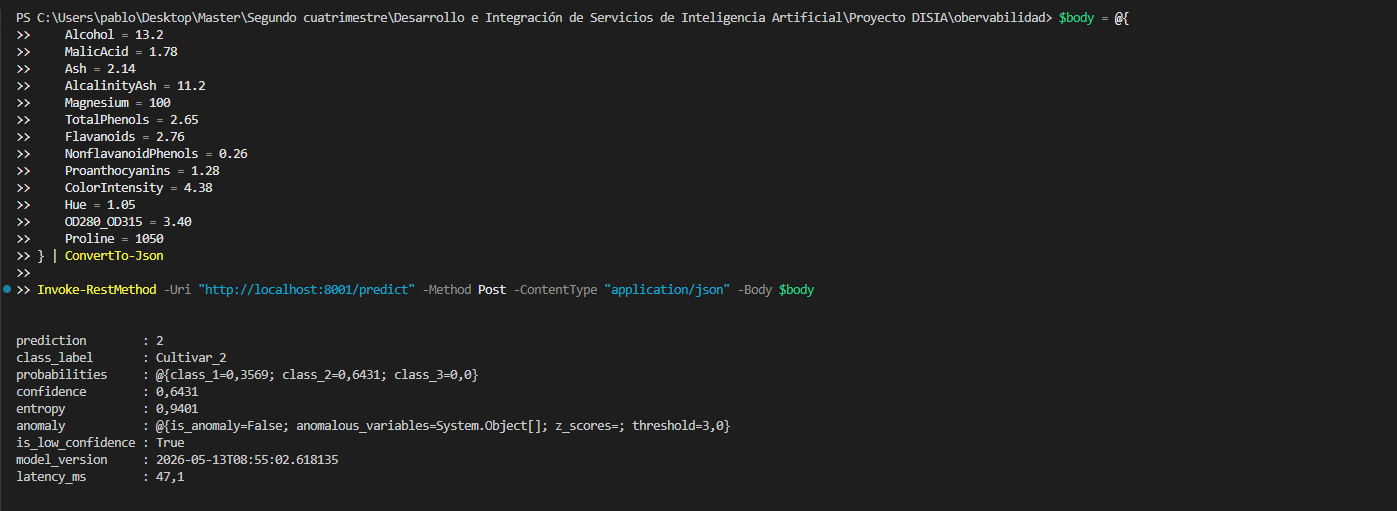
\includegraphics[width=0.88\textwidth]{Pictures/prediccion normal.png}
\caption{Ejemplo de predicción normal realizada por el endpoint \texttt{/predict}.}
\label{fig:h5_predict_normal}
\end{figure}

\begin{figure}[H]
\centering
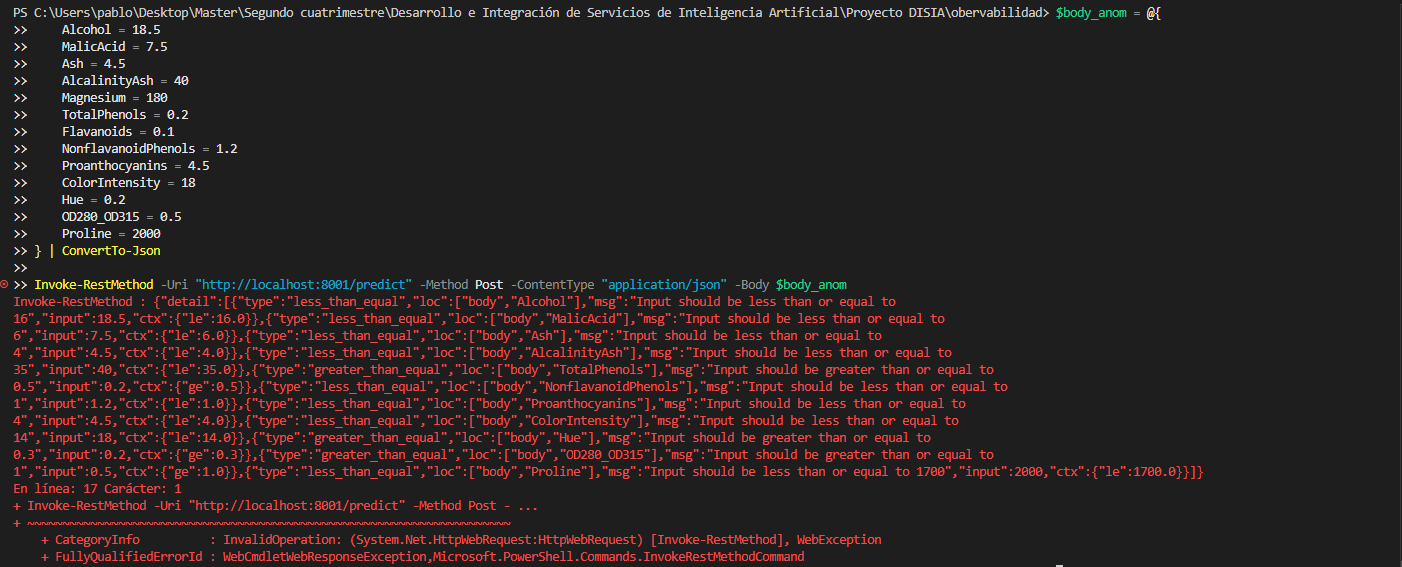
\includegraphics[width=0.88\textwidth]{Pictures/prediccion anomala.png}
\caption{Ejemplo de predicción anómala con indicadores activados en la respuesta del servicio.}
\label{fig:h5_predict_anomalous}
\end{figure}

\FloatBarrier

\section{Detección de drift y sistema de alertas}

Más allá de supervisar cada petición individual, el sistema necesita detectar cambios sostenidos en la distribución de los datos de entrada. En este contexto se ha optado por centrar el análisis en el \textit{data drift} o deriva de covariables, es decir, en el cambio de la distribución \(P(X)\) entre la fase de entrenamiento y la fase de operación. Esta elección resulta especialmente adecuada para VinOps porque puede evaluarse sin necesidad de disponer de la etiqueta real de cada muestra.

La Tabla \ref{tab:drift_tecnicas_hito5} presenta tres técnicas complementarias utilizadas en la implementación. En primer lugar, la prueba de Kolmogorov-Smirnov permite comparar distribuciones continuas de forma no paramétrica para cada variable individual. En segundo lugar, el \textit{Population Stability Index} proporciona una señal interpretable sobre la magnitud del desplazamiento entre distribuciones. En tercer lugar, la distancia de Wasserstein estandarizada ofrece una visión agregada del desplazamiento conjunto de la ventana observada.

\begin{table}[h]
\centering
\caption{Técnicas de detección de drift implementadas}
\vspace{0.2cm}
\begin{tabular}{l l l p{5.7cm}}
\hline
\textbf{Técnica} & \textbf{Tipo} & \textbf{Umbral} & \textbf{Finalidad principal} \\
\hline
Kolmogorov-Smirnov & Univariada & \(p < 0.05\) & Detectar cambios estadísticamente significativos en variables individuales. \\
PSI & Univariada & \(>0.10\) monitor, \(>0.25\) alerta & Medir estabilidad poblacional con una regla fácilmente interpretable. \\
Wasserstein & Multivariada & \(>1.0\) monitor, \(>2.0\) alerta & Capturar desplazamientos globales que podrían no apreciarse variable a variable. \\
\hline
\end{tabular}
\label{tab:drift_tecnicas_hito5}
\end{table}

Con el fin de equilibrar sensibilidad y coste computacional, se ha configurado una ventana deslizante de veinte muestras y una evaluación periódica cada diez predicciones. Esta decisión se justifica por el reducido tamaño del dataset original, ya que ventanas demasiado grandes introducirían una detección excesivamente lenta y ventanas demasiado pequeñas generarían señales muy ruidosas. La información de drift se resume mediante una regla jerárquica que diferencia entre estado normal, estado de monitorización y deriva detectada.

De forma simplificada, el sistema considera que existe deriva cuando se acumulan evidencias suficientes en varias variables o cuando el desplazamiento global medido por Wasserstein supera el umbral crítico. Esta combinación reduce el riesgo de falsos positivos debidos a fluctuaciones puntuales en una sola característica y aporta mayor robustez a la decisión global del monitor.

Sobre esta base se ha implementado un sistema de alertas por Telegram. Se eligió este canal por su simplicidad a la hora de integrarlo, por no requerir infraestructura propia y por resultar especialmente adecuado para una demostración en vivo, ya que permite visualizar las notificaciones de forma inmediata desde un chat. Además, el uso de variables de entorno para el token y el \texttt{chat\_id} evita exponer credenciales en el código fuente.

Con el objetivo de evitar saturación informativa, se ha incorporado un mecanismo de \textit{throttling} de sesenta segundos por tipo de alerta. Esta decisión reduce el riesgo de spam cuando una condición anómala persiste durante varios ciclos de monitorización, manteniendo al mismo tiempo una cadencia suficientemente frecuente para no perder capacidad de reacción.

Las alertas implementadas cubren dos familias de necesidades. Por un lado, se emiten alertas de modelo cuando se detecta drift, una tasa alta de anomalías o una caída sostenida de confianza media. Por otro lado, se generan alertas operativas cuando el servicio supera ciertos umbrales de CPU o memoria. A ello se añaden endpoints de simulación, como \texttt{/simulate/anomaly} y \texttt{/simulate/drift}, que permiten provocar escenarios controlados y verificar experimentalmente el funcionamiento del detector y del canal de notificación.

Con el fin de validar experimentalmente el sistema de monitorización, se ejecutaron simulaciones controladas que permitieron observar tanto la activación del canal de alertas como la actualización del estado de deriva del sistema. Las alertas enviadas por el bot de Telegram puede verse en las Figuras \ref{fig:h5_telegram_anomaly} y \ref{fig:h5_telegram_drift}, además del estado del estado del drift en la Figura \ref{fig:h5_drift_state}.

\begin{figure}[H]
\centering
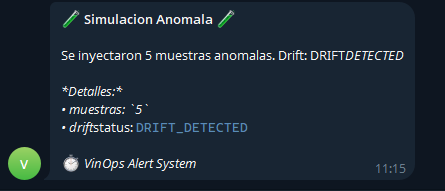
\includegraphics[width=0.78\textwidth]{Pictures/deteccion anomalia telegram.png}
\caption{Alerta enviada por Telegram tras detectar un comportamiento anómalo en el sistema monitorizado.}
\label{fig:h5_telegram_anomaly}
\end{figure}

\begin{figure}[H]
\centering
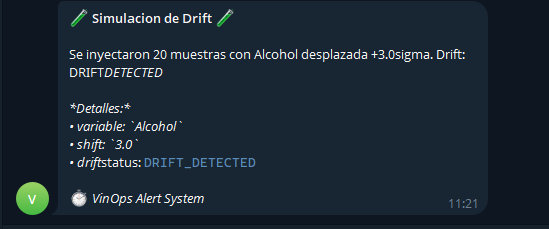
\includegraphics[width=0.78\textwidth]{Pictures/deteccion drift telegram.png}
\caption{Notificación de deriva enviada al canal de Telegram del proyecto.}
\label{fig:h5_telegram_drift}
\end{figure}

\begin{figure}[H]
\centering
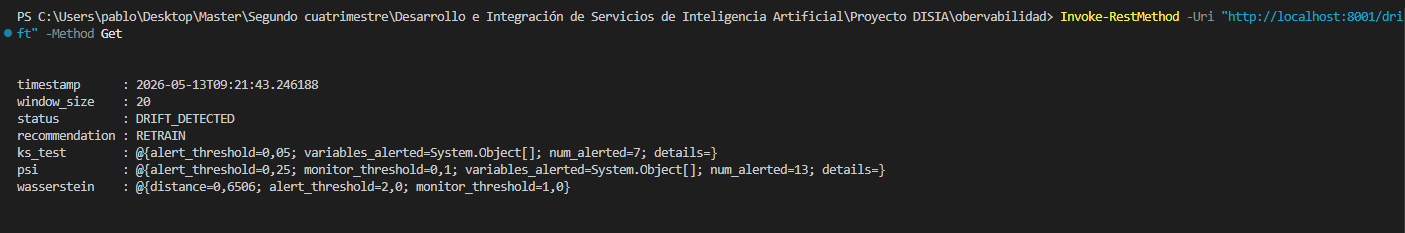
\includegraphics[width=0.85\textwidth]{Pictures/estado de drift.png}
\caption{Estado de drift del sistema tras la simulación, mostrando activación del monitor y recomendación de actuación.}
\label{fig:h5_drift_state}
\end{figure}

\FloatBarrier

\section{Visualización con Prometheus y Grafana}

La solución de visualización se ha articulado en tres capas. La primera capa corresponde a la propia API, que emite las métricas instrumentadas a través del endpoint \texttt{/metrics}. La segunda capa la constituye Prometheus, que scrapea periódicamente dichas métricas y las almacena como series temporales. Por último, Grafana consume esos datos y los presenta en un dashboard orientado a la monitorización del servicio.

El dashboard diseñado para el proyecto integra paneles dedicados a CPU, memoria, peticiones por segundo, latencia, confianza media del modelo, distribución de clases predichas, tasa de anomalías y entropía de predicción. Esta selección responde al objetivo de combinar indicadores operativos clásicos con señales específicas del comportamiento del clasificador, de modo que el operador disponga de una visión más completa del estado del sistema.

Una observación relevante durante las pruebas es que el uso de CPU aparece próximo a cero en condiciones normales. Este comportamiento no se debe a un error de instrumentación, sino a que el modelo empleado es muy ligero y la inferencia sobre un dataset pequeño apenas consume recursos en cada petición individual. En consecuencia, el valor del gauge solo crecería de forma apreciable bajo una carga artificialmente elevada.

La evidencia experimental de esta capa puede verse en las Figuras~\ref{fig:h5_prometheus_up} y~\ref{fig:h5_grafana_dashboard}.

\begin{figure}[H]
\centering
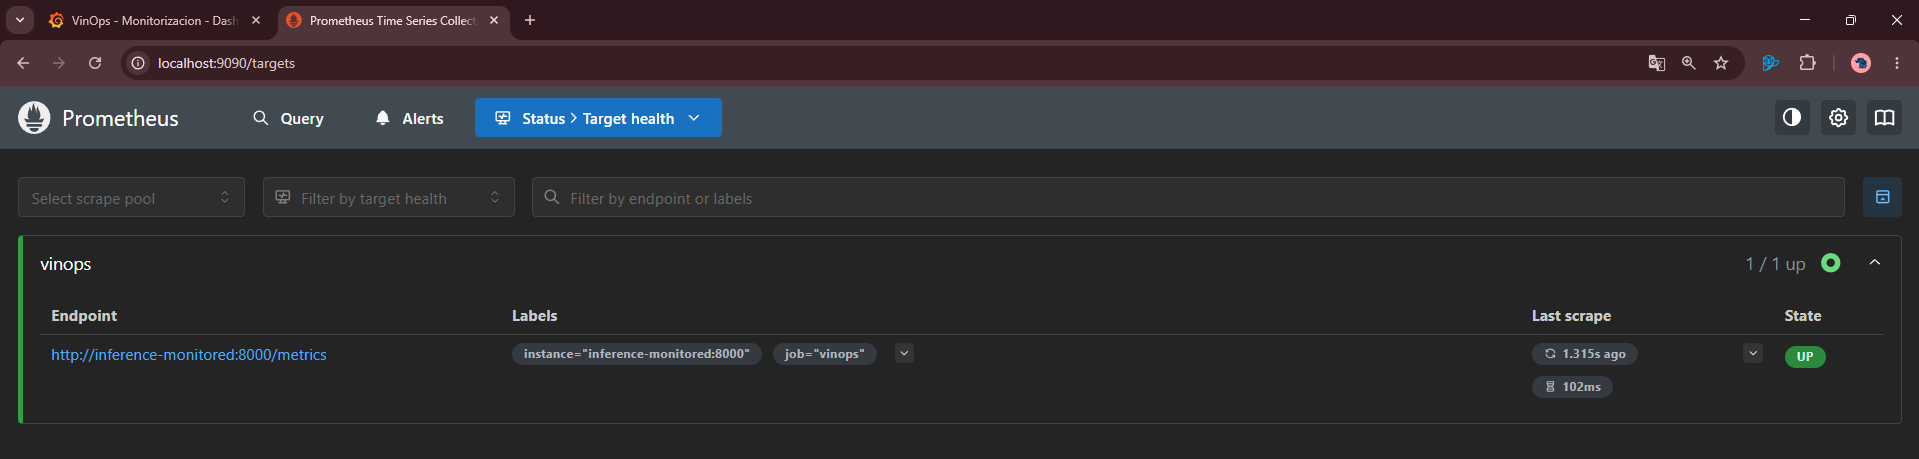
\includegraphics[width=0.95\textwidth]{Pictures/prometheus targets up.png}
\caption{Vista de Prometheus con el target del servicio en estado \texttt{UP}.}
\label{fig:h5_prometheus_up}
\end{figure}

\begin{figure}[H]
\centering
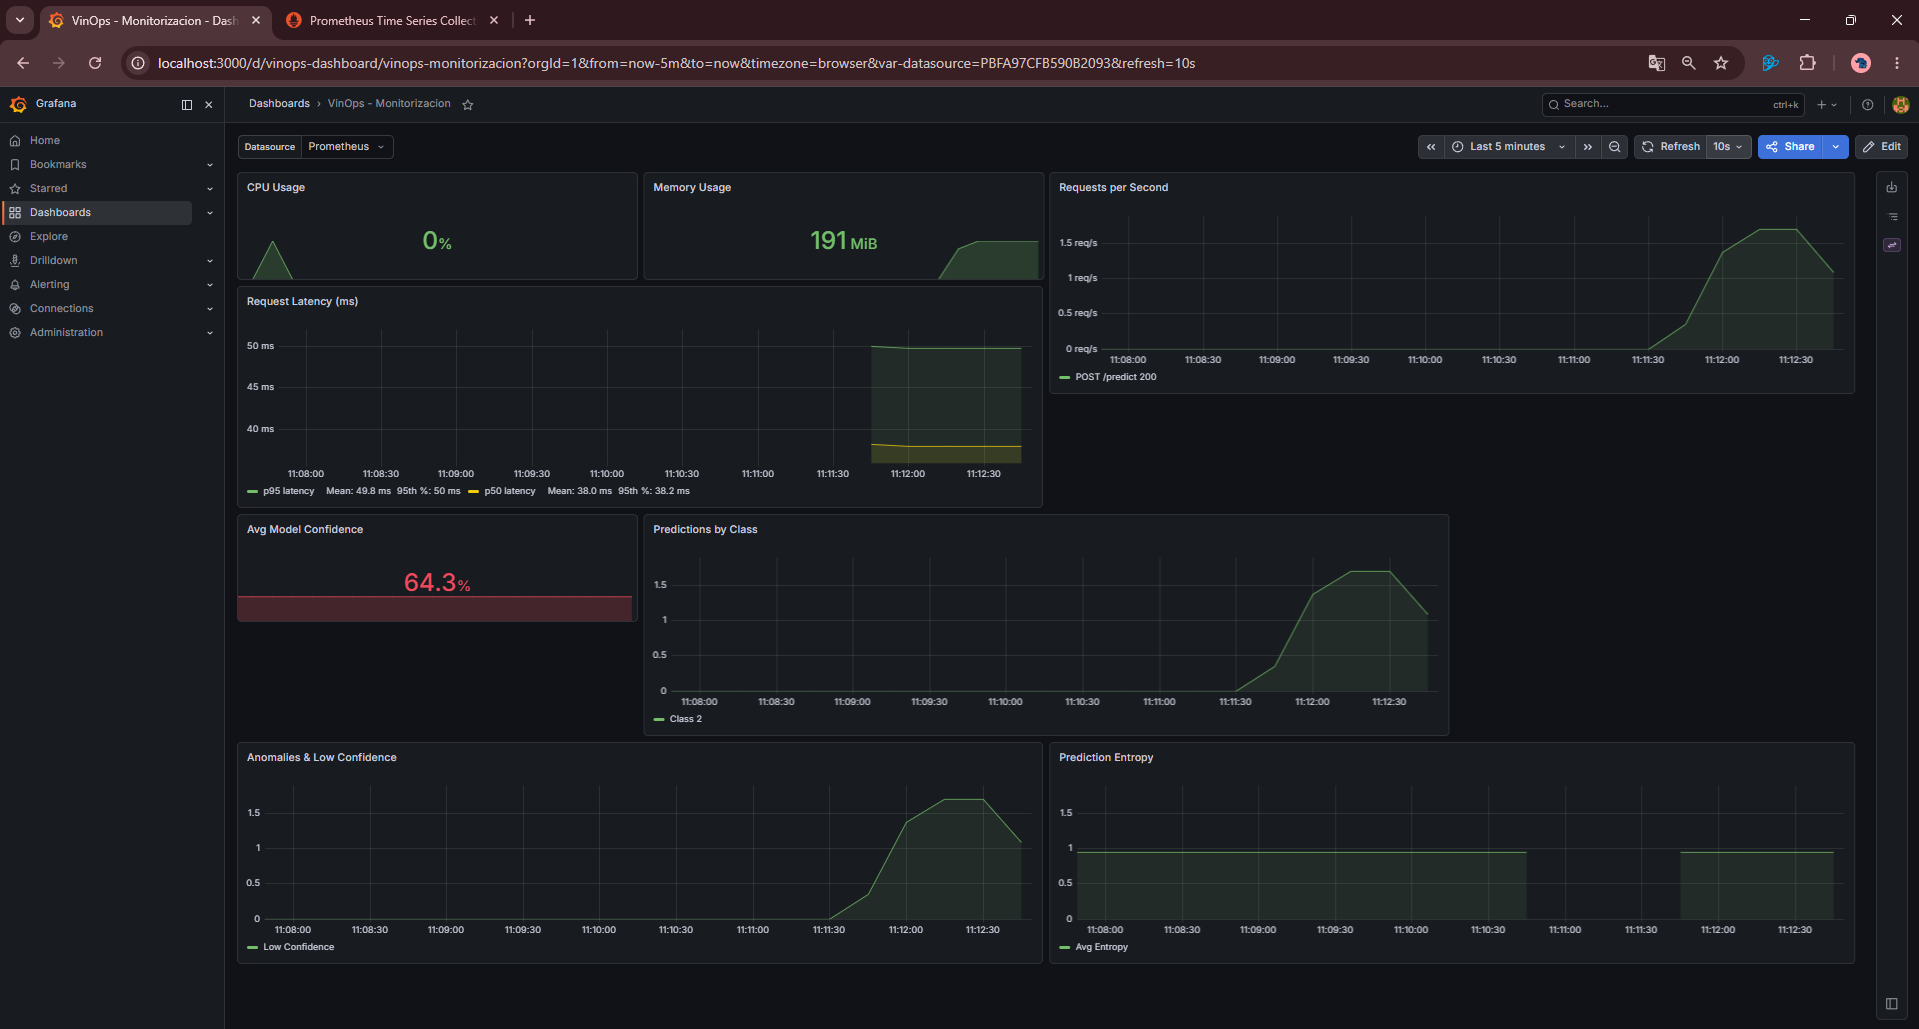
\includegraphics[width=0.98\textwidth]{Pictures/grafana dashboard.png}
\caption{Dashboard de Grafana con paneles de latencia, memoria, confianza y distribución de clases.}
\label{fig:h5_grafana_dashboard}
\end{figure}

\FloatBarrier

\section{Feedback loop y retraining semi-automático}

Uno de los elementos más importantes del Hito 5 es el cierre parcial del ciclo de vida del modelo mediante un mecanismo de feedback humano. La idea central consiste en permitir que el enólogo corrija predicciones una vez dispone de la etiqueta real, almacenando dichas correcciones para su uso posterior en un reentrenamiento supervisado. De este modo, el sistema no solo detecta degradación, sino que también incorpora una vía explícita para adaptarse a nuevos datos.

El diseño del trigger de reentrenamiento constituye una decisión relevante. En lugar de activar el retraining cuando se detecta un cierto número de eventos de drift, se ha optado por utilizar como criterio la acumulación de diez feedbacks reales. La razón es que el drift indica cambio en la distribución de entrada, pero no aporta por sí mismo la etiqueta correcta de las nuevas muestras. Sin \textit{ground truth}, un reentrenamiento supervisado carecería de base válida.

Las correcciones se almacenan en un archivo CSV en lugar de una base de datos relacional. Esta elección se justifica por la simplicidad del escenario, por el reducido volumen esperado de registros y por la facilidad con la que el archivo puede revisarse manualmente durante la evaluación académica. Aunque una base de datos ofrecería mejores garantías de escalabilidad y concurrencia, su incorporación habría añadido complejidad innecesaria para este contexto.

Otra decisión especialmente importante ha sido no reentrenar el modelo únicamente con las muestras corregidas. Dado que el dataset original contiene 178 observaciones, usar solo diez ejemplos de feedback conduciría a un riesgo elevado de sobreajuste y \textit{catastrophic forgetting}. Por este motivo, el sistema genera un dataset combinado formado por los datos originales más el feedback duplicado, otorgando así mayor peso a las correcciones recientes sin destruir el conocimiento aprendido previamente.

\[
\text{Dataset final} = \text{Original} + 2 \times \text{Feedback}
\]

En el caso evaluado, el conjunto original de 178 muestras se combina con diez correcciones duplicadas, produciendo un total de 198 observaciones para el reentrenamiento. Esta estrategia permite introducir adaptación al contexto operativo manteniendo al mismo tiempo una base suficientemente estable sobre la que apoyar la generalización del modelo. La duplicación del feedback se interpreta como una ponderación simple de las muestras recientes, no como generación de nuevas observaciones. En una versión productiva, esta ponderación debería parametrizarse y validarse empíricamente comparando distintos pesos del feedback.

Tras el reentrenamiento, el nuevo artefacto se recarga en memoria mediante el endpoint \texttt{/reload}, sin necesidad de reiniciar el contenedor. Esta decisión mejora la disponibilidad del sistema, preserva las métricas acumuladas por Prometheus y evita perder tanto la ventana de drift como el contexto operativo de la ejecución en curso.

La operativa del \textit{feedback loop} se validó mediante el envío manual de correcciones al endpoint \texttt{/feed\-back}, su persistencia en CSV y el posterior lanzamiento del proceso de reentrenamiento. Las Figuras~\ref{fig:h5_feedback_send}--\ref{fig:h5_reload} recogen la secuencia completa de corrección, almacenamiento, reentrenamiento y recarga del modelo.

\begin{figure}[H]
\centering
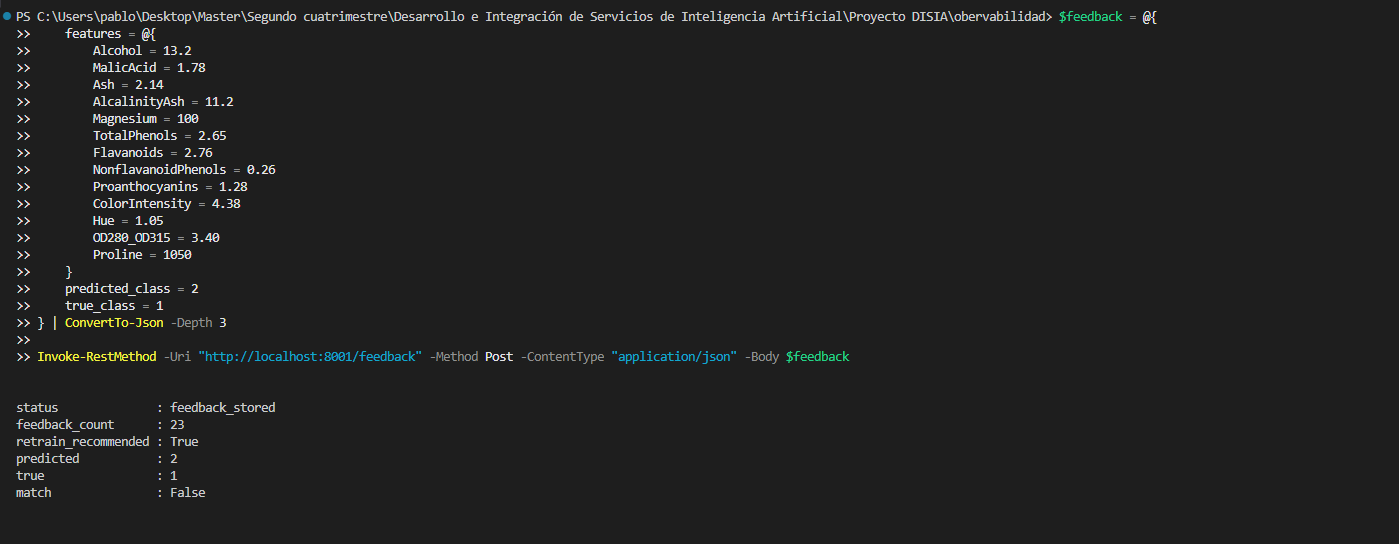
\includegraphics[width=0.86\textwidth]{Pictures/enviar feedback.png}
\caption{Registro de feedback manual enviado al sistema para alimentar el ciclo de mejora.}
\label{fig:h5_feedback_send}
\end{figure}

\begin{figure}[H]
\centering
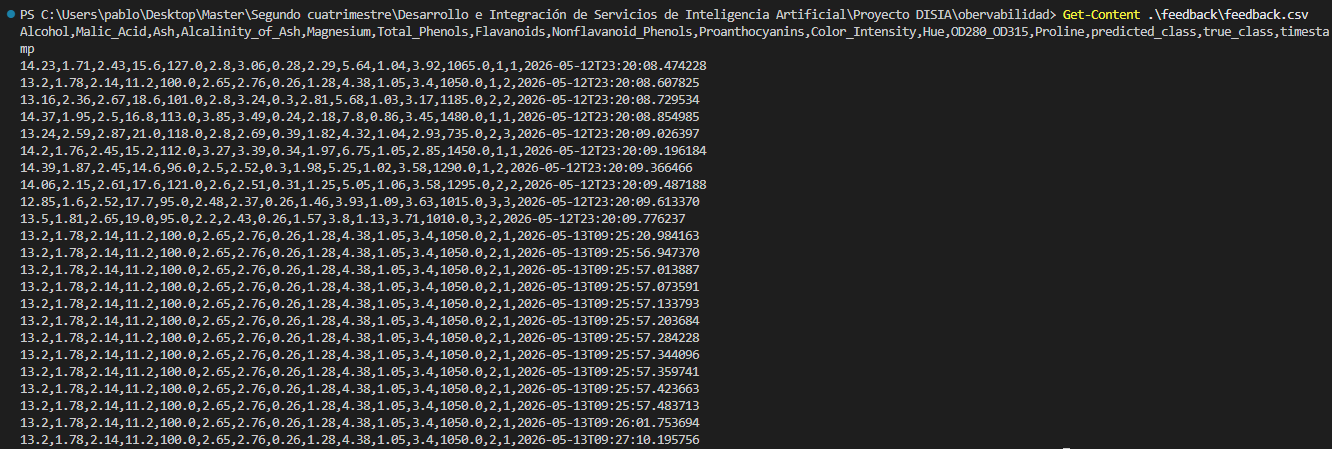
\includegraphics[width=0.90\textwidth]{Pictures/csv de feedback.png}
\caption{Persistencia del feedback acumulado en el archivo CSV del sistema.}
\label{fig:h5_feedback_csv}
\end{figure}

\begin{figure}[H]
\centering
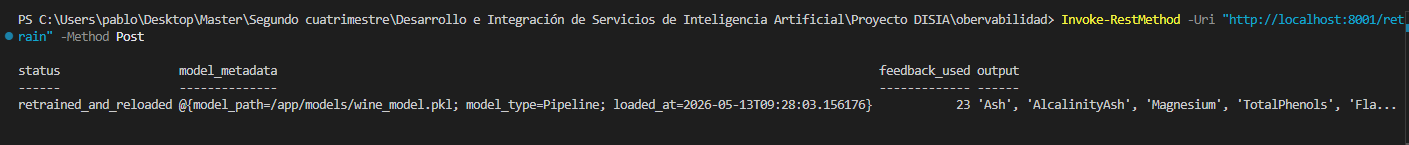
\includegraphics[width=0.84\textwidth]{Pictures/retraining.png}
\caption{Salida del endpoint \texttt{/retrain} mostrando la ejecución del reentrenamiento y sus resultados.}
\label{fig:h5_retraining}
\end{figure}

\begin{figure}[H]
\centering
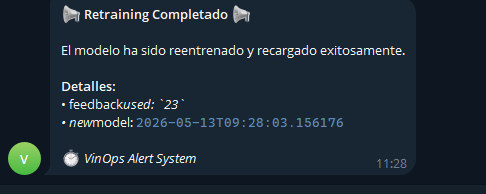
\includegraphics[width=0.75\textwidth]{Pictures/retraining telegram.png}
\caption{Notificación emitida tras la ejecución del proceso de reentrenamiento.}
\label{fig:h5_retraining_telegram}
\end{figure}

\begin{figure}[H]
\centering
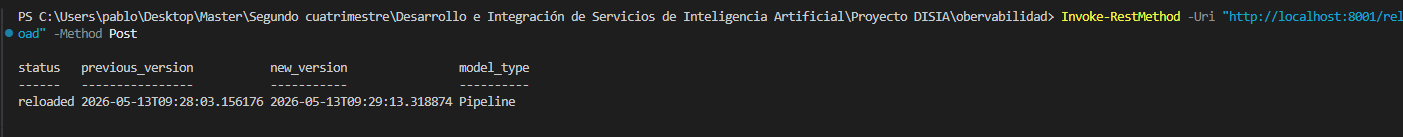
\includegraphics[width=0.84\textwidth]{Pictures/recarga sin reinicio.png}
\caption{Recarga del nuevo modelo en memoria mediante \texttt{/reload} sin reiniciar el contenedor.}
\label{fig:h5_reload}
\end{figure}

Los resultados obtenidos en el escenario descrito se resumen en la Tabla~\ref{tab:retraining_resultados}. Aunque se trata de una prueba académica y no de un proceso continuo real, el experimento demuestra la viabilidad del enfoque adoptado para cerrar parcialmente el ciclo de vida del modelo.

\begin{table}[h]
\centering
\caption{Resumen del retraining con feedback acumulado}
\vspace{0.2cm}
\begin{tabular}{l c}
\hline
\textbf{Elemento} & \textbf{Valor} \\
\hline
Dataset original & 178 muestras \\
Feedback acumulado & 10 muestras \\
Feedback tras duplicado & 20 muestras \\
Dataset combinado & 198 muestras \\
Macro F1-Score & 0.8757 \\
Balanced Accuracy & 0.8767 \\
\hline
\end{tabular}
\label{tab:retraining_resultados}
\end{table}

\FloatBarrier

\section{Bonus: shadow testing y comparación champion-challenger}

Como extensión opcional del hito, se ha implementado un mecanismo de \textit{shadow testing}, también denominado enfoque \textit{champion-challenger}. En este esquema, el modelo \textit{champion} continúa siendo el único que responde al cliente, mientras que un modelo \textit{challenger} recibe en segundo plano una copia de cada petición con el objetivo de comparar ambos comportamientos sin afectar al servicio principal.

Esta estrategia se ha preferido frente a un A/B testing clásico. La razón es que el A/B testing implicaría repartir el tráfico real entre dos modelos, lo que en un contexto académico y con un servicio todavía en evolución puede introducir riesgos innecesarios sobre la experiencia del consumidor. El shadow testing, en cambio, permite evaluar un candidato sin comprometer la respuesta operacional.

La implementación registra para cada petición la predicción del \textit{champion}, la del \textit{challenger}, la confianza asociada en ambos casos, el grado de acuerdo entre modelos y la latencia observada. Toda esta información se almacena en un CSV de comparaciones que permite inspeccionar posteriormente la consistencia del modelo candidato y su posible idoneidad para promoción.

Cuando el operador decide promover el challenger, el endpoint \texttt{/shadow/promote} sustituye el artefacto activo por el modelo candidato y actualiza la instancia cargada en memoria. De este modo, la transición puede realizarse sin reiniciar el contenedor y manteniendo la continuidad operativa del servicio.

Las Figuras~\ref{fig:h5_bonus_health}--\ref{fig:h5_shadow_promote} muestran la validación experimental completa del flujo champion-challenger.

\begin{figure}[H]
\centering
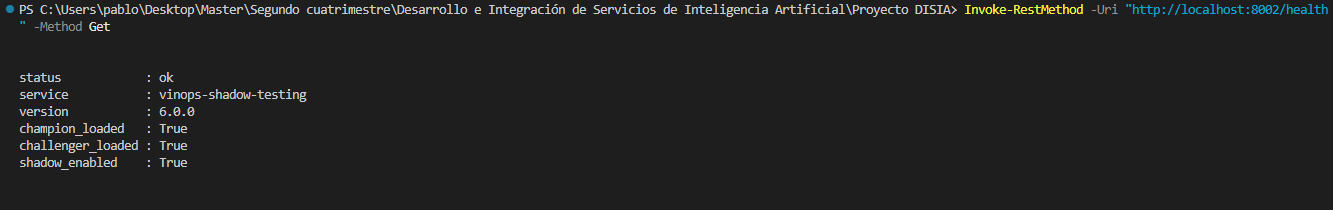
\includegraphics[width=0.82\textwidth]{Pictures/health del bonus.png}
\caption{Respuesta del endpoint \texttt{/health} del entorno bonus de shadow testing en el puerto 8002.}
\label{fig:h5_bonus_health}
\end{figure}

\begin{figure}[H]
\centering
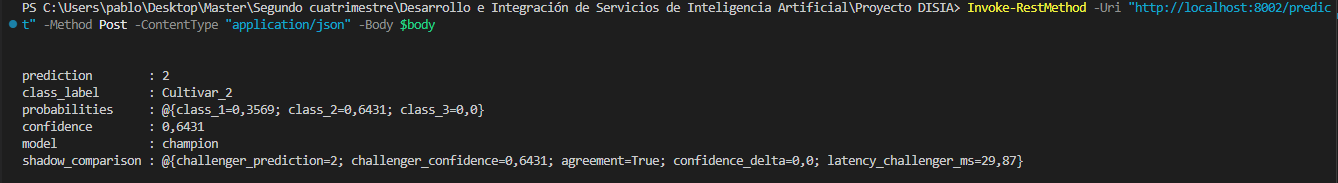
\includegraphics[width=0.88\textwidth]{Pictures/prediccion champion-challenger.png}
\caption{Predicción en modo champion-challenger con comparación entre ambos modelos.}
\label{fig:h5_shadow_predict}
\end{figure}

\begin{figure}[H]
\centering
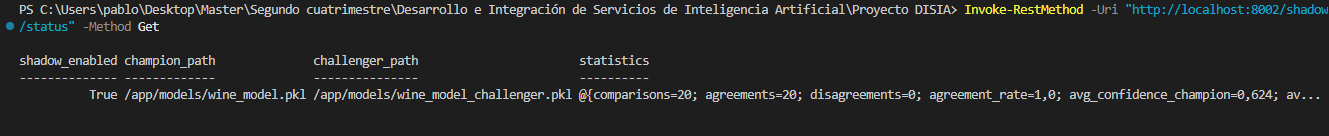
\includegraphics[width=0.82\textwidth]{Pictures/estado shadow.png}
\caption{Estado agregado del shadow testing con métricas de comparación entre champion y challenger.}
\label{fig:h5_shadow_status}
\end{figure}

\begin{figure}[H]
\centering
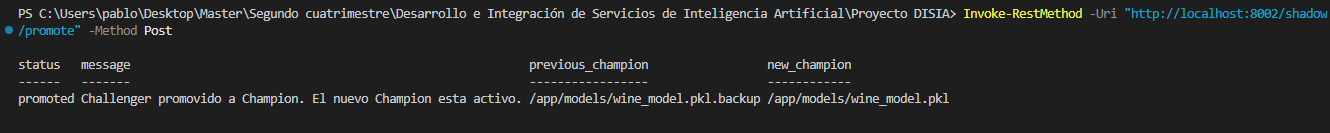
\includegraphics[width=0.82\textwidth]{Pictures/promocion del challenger.png}
\caption{Promoción del modelo challenger a champion mediante el endpoint \texttt{/shadow/promote}.}
\label{fig:h5_shadow_promote}
\end{figure}

\FloatBarrier

\section{Decisiones de diseño globales}

A lo largo del desarrollo del hito se han adoptado varias decisiones con impacto directo sobre la arquitectura y la operatividad del sistema. La Tabla~\ref{tab:decisiones_hito5} resume las principales elecciones, la alternativa descartada en cada caso y la justificación asociada.

\begin{table}[h]
\centering
\caption{Decisiones de diseño principales del Hito 5}
\vspace{0.2cm}
\begin{tabular}{p{3.5cm} p{4cm} p{6.2cm}}
\hline
\textbf{Decisión} & \textbf{Alternativa descartada} & \textbf{Justificación} \\
\hline
Métricas proxy online & F1, precisión o AUC en tiempo real & La etiqueta real no está disponible en el momento de la predicción. \\
Implementación estadística ligera & Frameworks como Alibi Detect o NannyML & Se prioriza un contenedor más manejable y una solución comprensible en contexto académico. \\
CSV para feedback & SQLite o PostgreSQL & El volumen esperado es pequeño y el archivo resulta fácil de inspeccionar. \\
Retraining con originales + feedback duplicado & Reentrenar solo con feedback & Se reduce el riesgo de sobreajuste y de olvido catastrófico en small data. \\
Trigger de 10 feedbacks & Trigger por eventos de drift & El drift no aporta por sí mismo etiquetas válidas para aprendizaje supervisado. \\
Telegram como canal de alertas & Correo o plataformas corporativas & La integración es simple y la demostración resulta más visible e inmediata. \\
Recarga en caliente & Reinicio del contenedor & Se evita downtime y se preserva el estado operativo. \\
Shadow testing & A/B testing & Permite evaluar modelos candidatos sin afectar al tráfico servido. \\
\hline
\end{tabular}
\label{tab:decisiones_hito5}
\end{table}

Las implicaciones de estas decisiones son ambivalentes. Por un lado, el sistema gana claridad, trazabilidad y facilidad de despliegue en un entorno académico. Por otro, algunas elecciones priorizan la simplicidad frente a la escalabilidad, por lo que en un entorno productivo real sería razonable evolucionar hacia soluciones con versionado de modelos, almacenamiento más robusto y mecanismos automáticos de rollback.

\section{Limitaciones y valoración final del hito}

A pesar de los avances alcanzados, la solución implementada presenta varias limitaciones. En primer lugar, el modelo reentrenado sobrescribe el artefacto anterior, por lo que no existe aún un versionado formal ni un mecanismo automático de reversión. En segundo lugar, el feedback utilizado para reentrenar no queda marcado como consumido, lo que podría complicar su trazabilidad si el sistema evolucionara hacia un uso continuado. Finalmente, el entorno de shadow testing se ha planteado como una validación controlada, por lo que su valor demostrativo es mayor que su madurez operativa real.

No obstante, el Hito 5 supone un avance cualitativo importante respecto a los hitos anteriores. El proyecto deja de ser únicamente un modelo desplegado y pasa a incorporar varios elementos esenciales de observabilidad y ciclo de vida MLOps: métricas operativas, métricas proxy del modelo, detección de drift, alertas automáticas, feedback humano, reentrenamiento supervisado y comparación segura entre modelos.

En conjunto, las decisiones adoptadas incrementan la complejidad estructural del sistema respecto al Hito 4, pero lo hacen a cambio de una mejora clara en su capacidad de supervisión, adaptación y explotación. Aunque se trata todavía de una solución local y académica, el resultado aproxima el proyecto a un escenario real de operación y sienta una base razonable para futuras extensiones como MLflow, auto-retraining, canary deployment o estimación avanzada de degradación sin \textit{ground truth}.